\chapter{Results}
\label{chap:results}

% section intro
In this chapter, we show the experimental results of the above discussed algorithms.
We compare them to a baseline called \algRand{}, where the principal chooses which subsets to reveal uniformly at random from the as of yet unrevealed subsets.
In all experiments, the initially known subsets $ \k $ are simply the minimal information $ \k_0 $.

% experimenty jsou i z clankuu
We first show results utilizing the game-theoretic motivation, with the utopian gap (\Cref{def:gap}) set as the divergence.
These results are already published by \cite{uradnik2024reducing}, along with a very well-performing heuristic for uniform distribution over monotone supermodular games.
In this thesis, we extend these results for different divergence functions, utilizing the $ L_k $-norms.
We compare these results to those with the utopian gap.
Finally, we show some examples documenting properties of the divergence already discussed above.

% Metacentrum technical info
The code for conducting the experiments was written in Python~3.10 using \texttt{stable\_baselines3}~2.0 \citep{stable-baselines3}, \texttt{gymnasium}~0.28 \citep{towers_gymnasium_2023} and \texttt{pytorch}~2.0 \citep{Ansel_PyTorch_2_Faster_2024}, and is available at Github \citep{gitrepo}.
We ran all experiments on a cluster with AMD~EPYC~7532~CPUs running at 2.4~GHz.
When running the experiments, we utilized 15~cores and 12~GB of RAM.

\section{Experimental Domains}

In this section, we explore different distributions of set functions/cooperative games and see how our methods compare for different choices of the budget $ \tau $ and the divergence function $ \ell $.
As we have shown in \Cref{thm:algfo-time-complexity-double-exp}, the time complexity of the optimal variants of the algorithms is double-exponential in the size of the ground set $ n $ for a sufficiently large budget $ \tau $.
For this reason, we only present the results for $ n=5 $, for which the results for each of the optimal algorithms took approximately 1,000 CPU hours to compute.
Using the complexity bound from \Cref{thm:algfo-time-complexity-double-exp}, we estimate that for $ n=6 $, to obtain similar results for the optimal algorithms  would require over 1,000 CPU years with the computational resources currently available to us.

There are countless options to choose from for the divergence function $ \ell $.
In this thesis, we focus on the performance of our algorithms with the utopian gap as divergence (\Cref{def:gap}), because it is well motivated in cooperative game theory.
We further show the performance with the $ L_1 $ and $ L_2 $ norms as divergence functions.
These are very general, not tied to a specific application, and they have a geometric interpretation which ties them to the original motivation of the divergence---to measure the size of the set of superadditive extensions.
See \Cref{sec:divergence} for more details.
As we will see, the results are similar for the two $ L_k $ norms, and we hypothesize that this is also the case for larger $k$.

\subsection{Factory Game}

% factory game class
The first setting  we focus on is a class of cooperative games we call the \emph{factory games}.

\begin{defi}[Factory game]
  Let $ N = \left\{ 1, \ldots, n \right\} $ be a set of players and $ o \in N $ be an \emph{owner}.
  Then a \emph{factory game} has a characteristic function $ v_o $ defined as \[
    \fce{v_o}{S} \deq \begin{cases}
      \absolute{S} - 1 & \text{if $ o \in S $,} \\
      0                & \text{otherwise.}
    \end{cases}
  \]
\end{defi}

This game is a very simple model of a factory, with $ n-1 $ equally productive workers, and one owner of the factory.
If the owner is present in a coalition, the workers can work in the factory, each producing a value of $ 1 $.
Otherwise, the workers cannot work, and thus produce nothing.

The point of this example is not to precisely model a real-world situation.
It is rather to have a finite class of superadditive games with very simple structure, on which we can thus run our algorithms and compare their performance.

\begin{figure*}[t!]
  \centering
	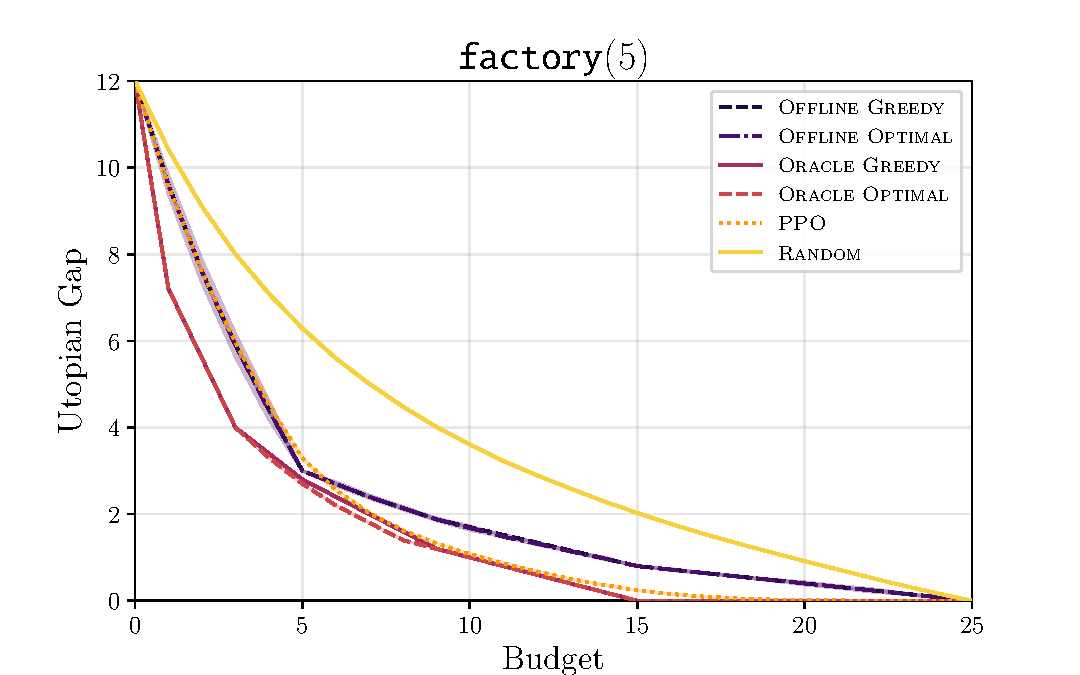
\includegraphics[width=\stdfigwidth]{figures/exploitability_predictible_factory5.pdf}
	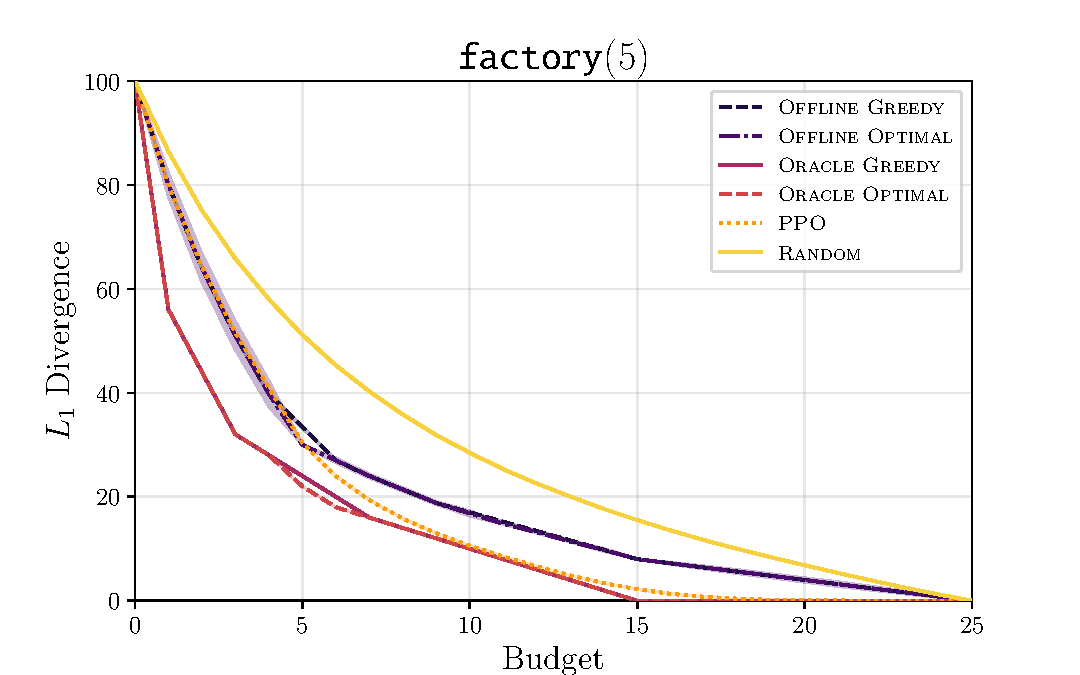
\includegraphics[width=\stdfigwidth]{figures/l1_norm_predictible_factory5.pdf}
	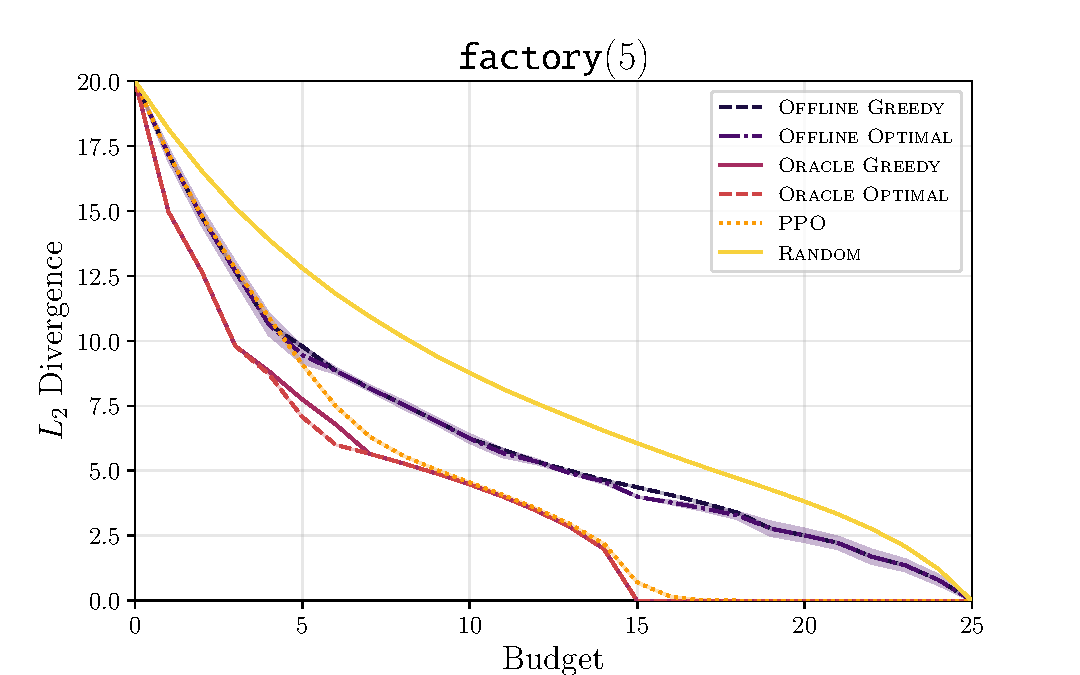
\includegraphics[width=\stdfigwidth]{figures/l2_norm_predictible_factory5.pdf}
	\caption{ The divergence as a function of budget $ \tau $ on the $ \factory[5] $ distribution for the utopian gap \citep[][Figure 1]{uradnik2024reducing} and the $ L_1 $- and $ L_2 $-divergence.}
	\label{fig:factory}
\end{figure*}
\begin{figure*}[t!]
  \centering
	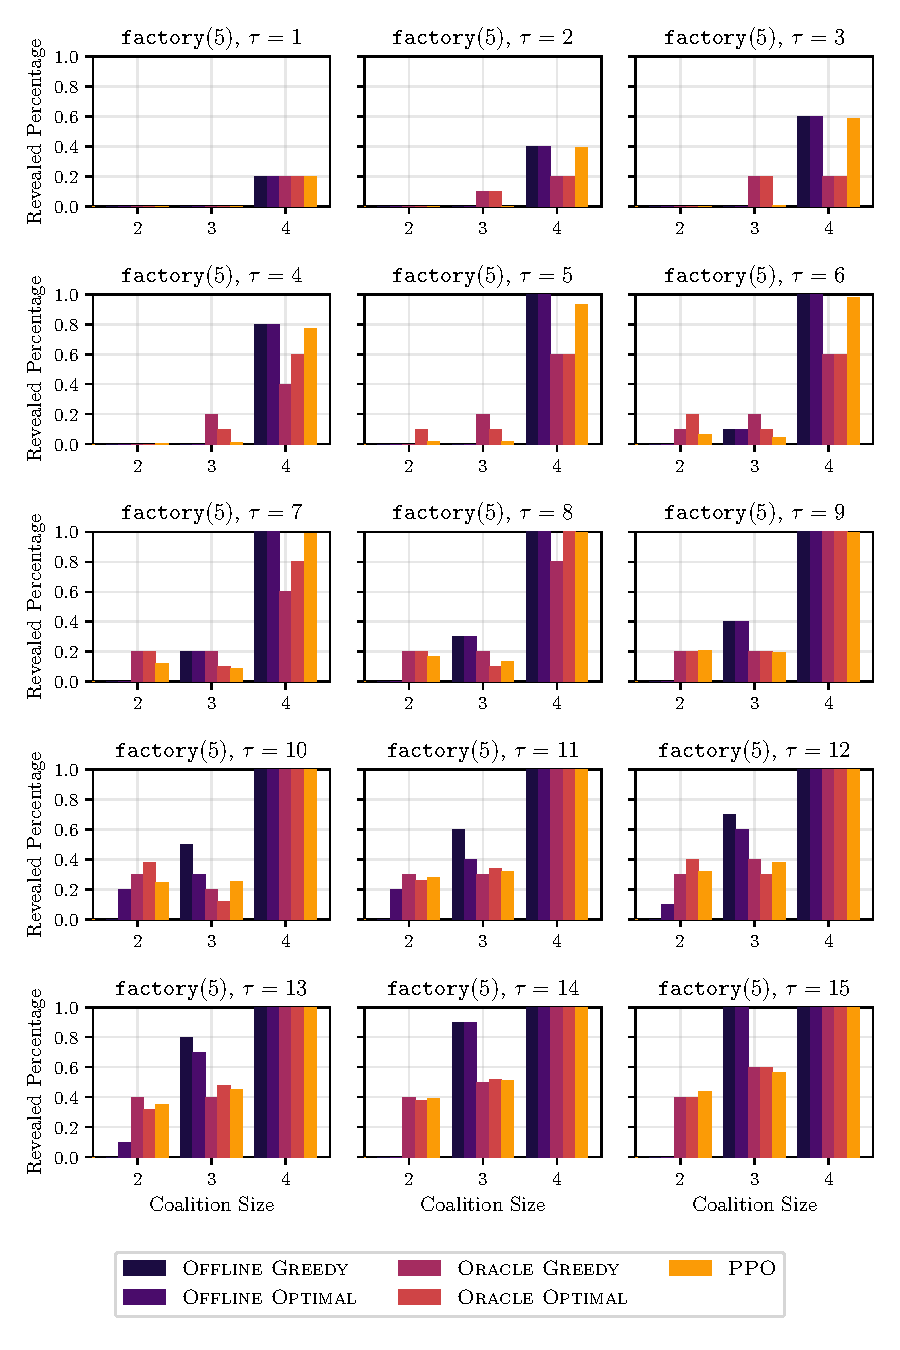
\includegraphics[width=\textwidth]{figures/exploitability_predictible_factory5_coalition_bar_sizes.pdf}
	\caption{ The percentage of subsets of a given size revealed in steps $1 $ to $ 15$ for the different approaches, when ran on the $\factory[5]$ distribution with $L_1$-divergence.
	Similar results can be seen for the $ L_2 $-divergence and the utopian gap (see \Cref{app:subsets}). }
	\label{fig:factory_coals}
\end{figure*}

% factory distribution
For a given $ n \in \N $, there are $ n $ different factory games, each with a different owner.
When running the experiments, we choose $ \fdist $ to be a uniform distribution on these $ n $ games, which we denote as $ \factory $.
\Cref{fig:factory} shows the results of our experiments for $ n=5 $ as a function of the budget $ \tau $, for different choices of divergence functions.

% explain the observed
For all three version of the divergence functions we studied, all our proposed algorithms outperform the \algRand{} approach.
Further, both the offline algorithms are significantly outmatched by their oracle variants.
The PPO algorithm starts off close to the offline algorithms, since for a small budget, it does not yet have any additional information about the function.
As the budget grows, and PPO gains more information about the specific game (in this case, information about which player is the owner), it begins to noticeably outperform the offline algorithms, and approaches the oracle algorithms.

\Cref{fig:factory_coals} shows the percentage of subsets (coalitions) of a given size revealed at steps $ \tau= 1 $ to $ 15 $ by each algorithm.
Initially, the best strategy is to reveal the biggest subsets.
The algorithms differ only in their ordering---the oracle algorithms first choose the one where the owner is missing, while the rest, not knowing who the owner is, must choose at random.
The offline algorithms continue on to reveal the coalitions of size $ 3 $, while the oracle algorithms use their knowledge of the owner to reveal some coalitions of size 2 and some of size 3, reaching zero gap at $ \tau=15 $.
PPO, having performed a strategy which mimics the offline algorithms for $ \tau \leq 5 $, now closely follows the oracle algorithms, also achieving near-zero gap at $ \tau=15 $.

% comparison of divergence functions
Now, let us compare the utopian gap and the $ L_1 $-divergence, shown also in \Cref{fig:factory}.
The performance of all algorithms is almost identical to the performance for the utopian gap.
This is due to the fact that the Shapley value, which is what the utopian gap uses when computing divergence, is a linear combination of the values of all coalitions.
The utopian gap is then naturally very similar to the $ L_1 $ norm, where each term has a weight with which it contributes to the divergence.

\Cref{fig:factory} further shows the performance of our algorithms under the $ L_2 $-divergence.
Compared to $ L_1 $, the $ L_2 $ norm gives more weight to the subsets where the difference between the upper and lower bound is greater.
This property further encourages the algorithms to reveal the values of largest subsets first, as they initially contribute the most to the divergence.
However, the relative performance of each algorithm does not change significantly as compared to the $ L_1 $-divergence.
Interestingly, the difference between the performances of the offline and oracle approaches seems to be slightly widening---the knowledge of the owner is even more valuable, as it allows closing the biggest differences faster.
Again, this shows that the PPO algorithm starts off behaving similarly to the offline approaches, and reaches the performance of the oracle approaches as the budget increases.

\begin{figure*}[t!]
  \centering
	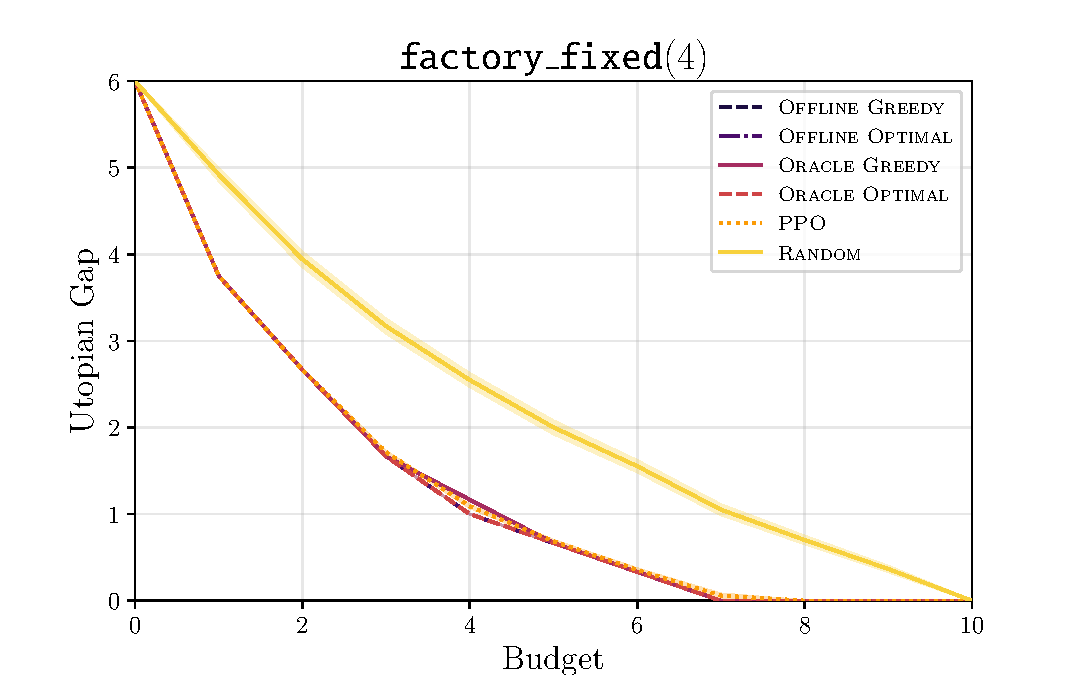
\includegraphics[width=\stdfigwidth]{figures/exploitability_factory_fixed4.pdf}
	\caption{ The divergence as a function of budget $ \tau $ on the $ \factoryf[4] $ distribution for the utopian gap \citep[][Figure 4]{uradnik2024reducing}.}
	\label{fig: fixed owner factory}
\end{figure*}

% greedy ain't optimal
Let us now focus on the differences between the performance of the greedy and optimal algorithms.
We have not yet discussed whether the greedy algorithms behave optimally, or if there is a difference between the performance of greedy and optimal algorithms.
This is best illustrated in \Cref{fig: fixed owner factory}, where an altered distribution over the factory games is used, always yielding the game with player 1 as the factory owner.
This distribution, which we denote as $\factoryf$, has support size of one, and thus the offline algorithms become identical to the oracle algorithms.
While the greedy and optimal algorithms are close to each other, at step $ \tau = 5 $, the optimal algorithms are in fact strictly better than their greedy counterparts.
A detailed view of the subsets chosen at each step is available in \Cref{app:subsets}.

\subsection{Supermodular}

% remind what supermodular is
The class of supermodular functions is widely studied in many fields, most notably in economics and cooperative game theory \citep{grabisch2016set,doi:10.1287/ijoc.15.3.284.16077}.
It has a very rich structure, and many interesting properties \citep{Lovasz1983}.
Our experiments were conducted on a uniform distribution of monotone supermodular games on $ n $ elements, where the ground set has unit value.
We denote this distribution as $ \supermodular $.
To conduct our experiments, we use an efficient algorithm for sampling from such a distribution \citep{9252865}.
The results of those experiments for $ n=5 $ are presented in \Cref{fig:supermodular}.

\begin{figure*}[t!]
  \centering
	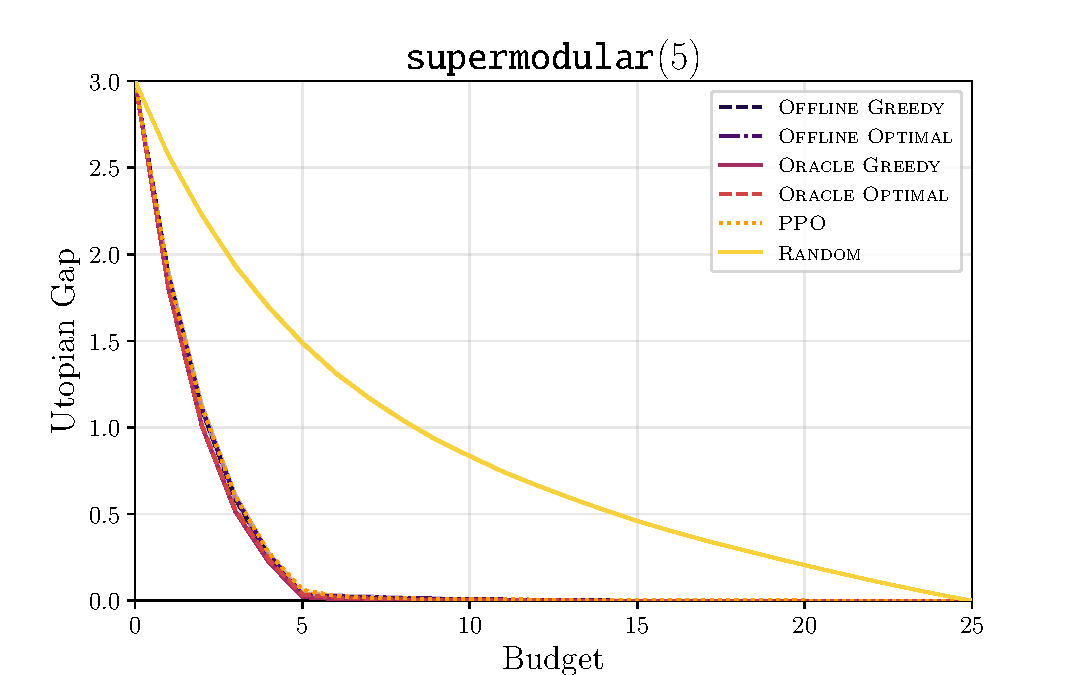
\includegraphics[width=\stdfigwidth]{figures/exploitability_convex5.pdf}
	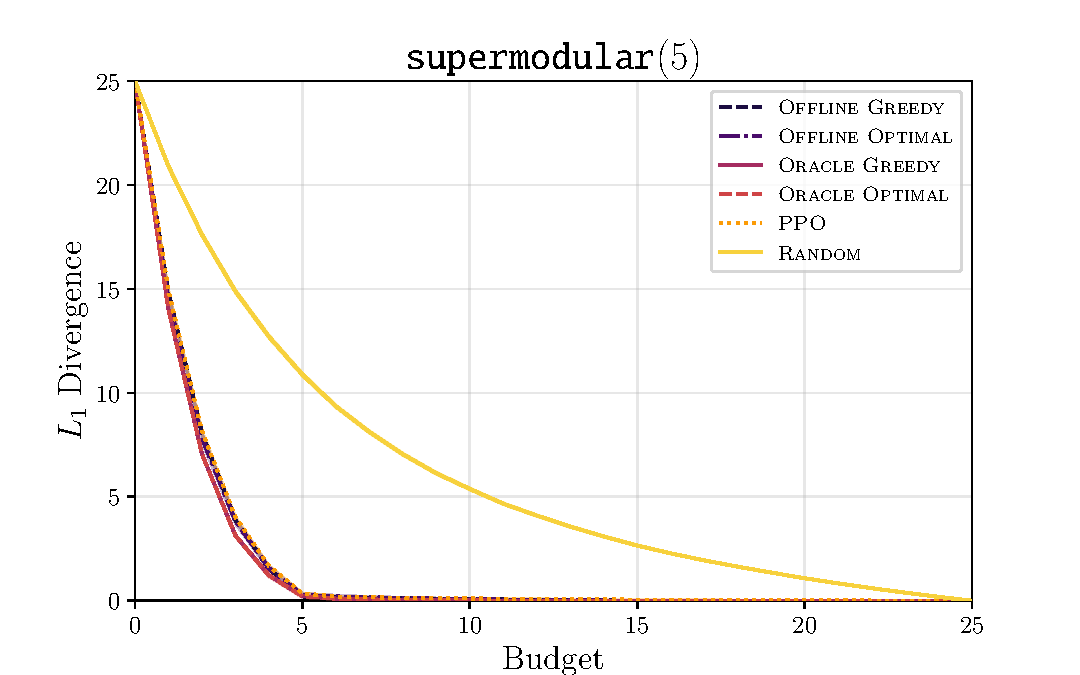
\includegraphics[width=\stdfigwidth]{figures/l1_norm_convex5.pdf}
	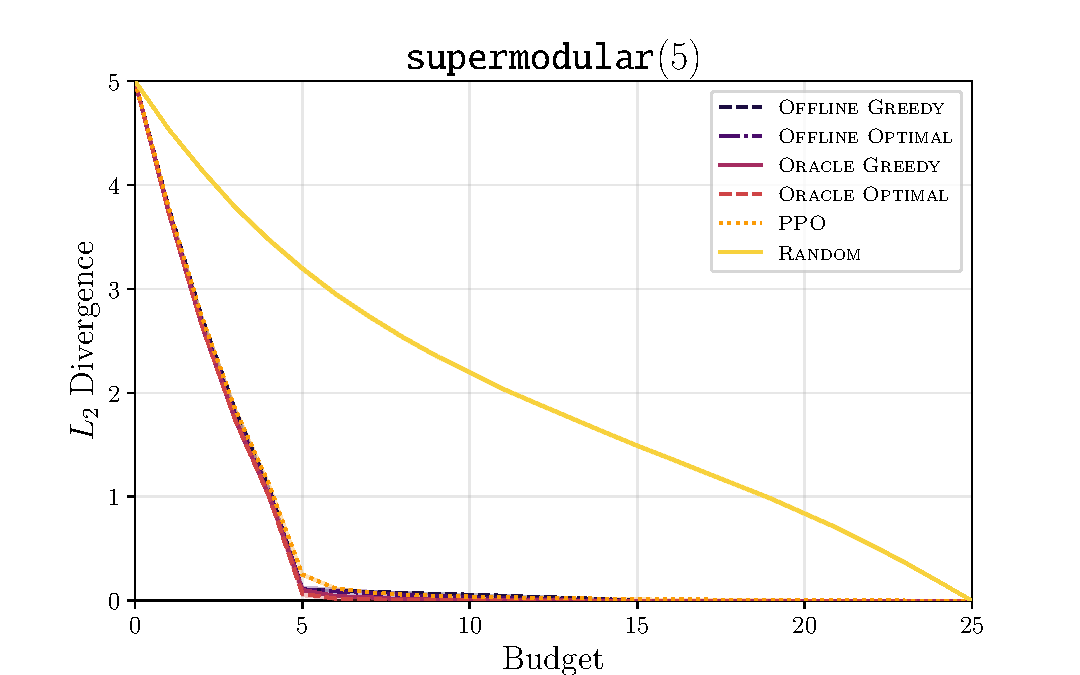
\includegraphics[width=\stdfigwidth]{figures/l2_norm_convex5.pdf}
	\caption{ The divergence as a function of budget $ \tau $ on the $ \supermodular[5] $ distribution for the utopian gap \citep[][Figure 1]{uradnik2024reducing} and the $ L_1 $- and $ L_2 $-divergences.}
	\label{fig:supermodular}
\end{figure*}

\begin{figure*}[t!]
  \centering
	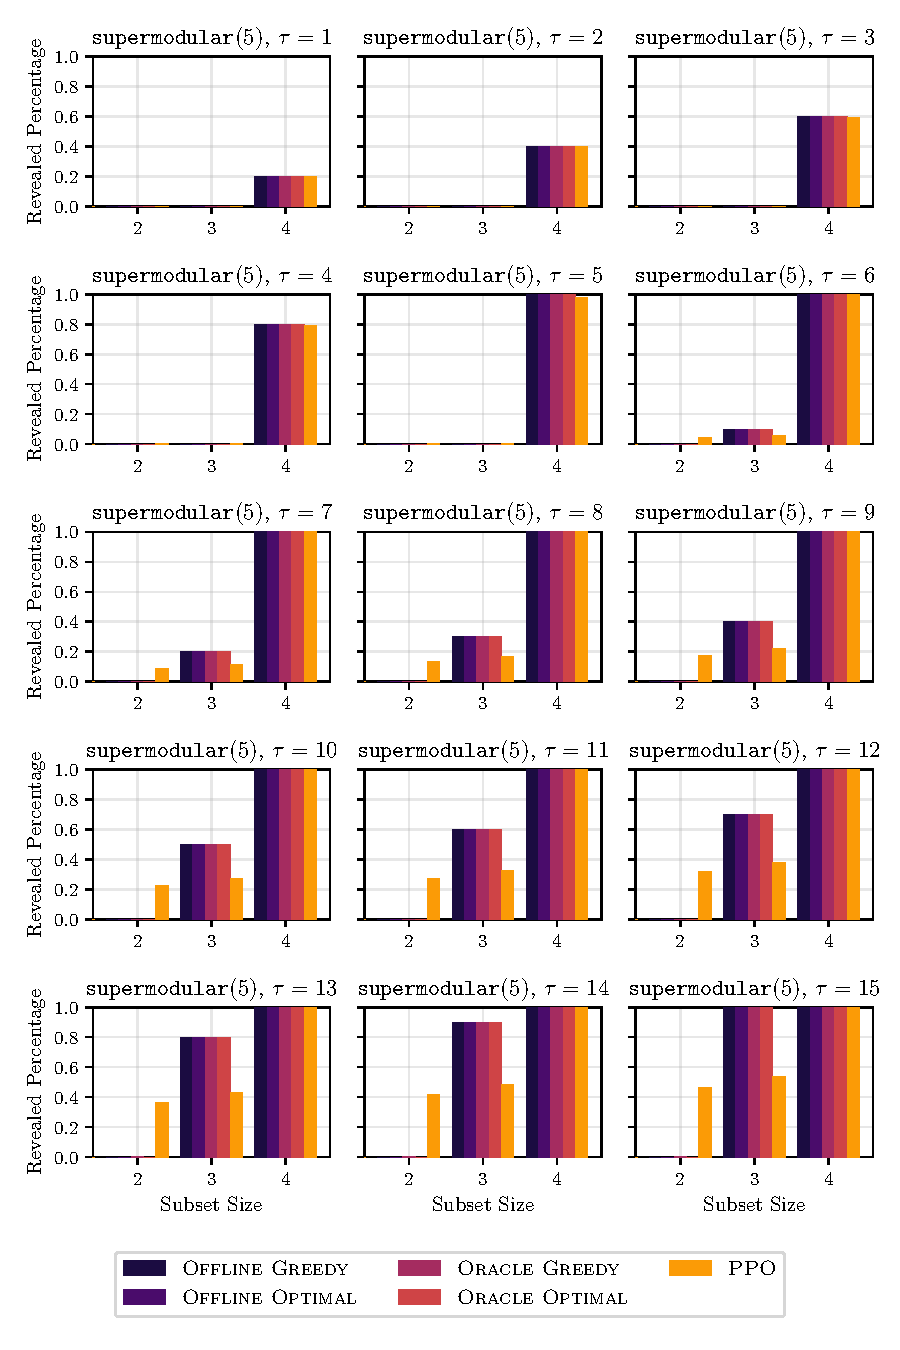
\includegraphics[width=\textwidth]{figures/l1_norm_convex5_coalition_bar_sizes.pdf}
	\caption{ The percentage of subsets of a given size revealed in steps $1 $ to $ 15$ for the different approaches, when ran on the $\supermodular[5]$ distribution with $L_1$-divergence.
	  Similar results can be seen for the $ L_2 $-divergence and the utopian gap (see \Cref{app:subsets}). }
	\label{fig:supermod_coals}
\end{figure*}

% explain the observed
Surprisingly, our algorithms work remarkably well on the $ \supermodular[5] $ distribution for all our three choices of the divergence function.
All algorithms vastly outperform the \algRand{} approach, reducing the divergence by over 99\% with just the budget of $ \tau = 5 $.
Furthermore, all our algorithms exhibit very similar performance, suggesting that the knowledge of the specific function drawn from the distribution is of little help when decreasing the divergence.
To illustrate the strategy used by each algorithm, \Cref{fig:supermod_coals} shows the distribution of revealed subsets for steps $\tau= 1 $ to $ 15 $.
We investigate these findings further in \Cref{ssec:largest}.

\section{Offline vs. Oracle}
\label{sec:linf}

\begin{figure*}[t!]
  \centering
	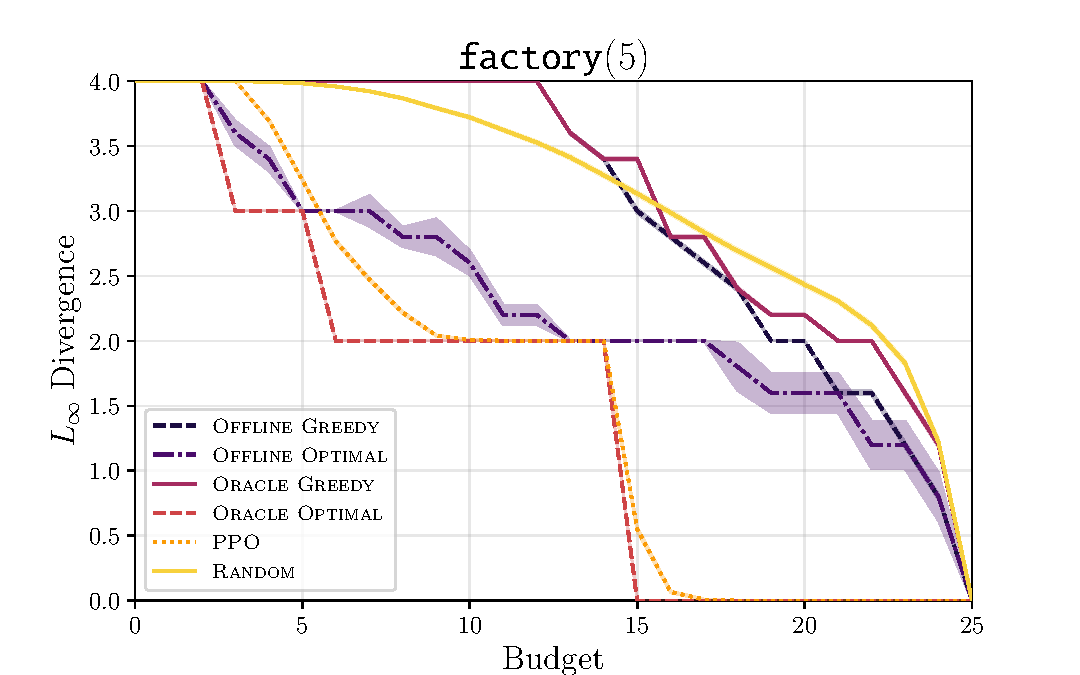
\includegraphics[width=\stdfigwidth]{figures/linf_norm_predictible_factory5.pdf}
	\caption{ The divergence as a function of budget $ \tau $ on the $ \factory[5] $ distribution for the $ L_\infty $-divergence. }
	\label{fig:offlinebeatsoracle}
\end{figure*}

\begin{figure*}[t!]
  \centering
	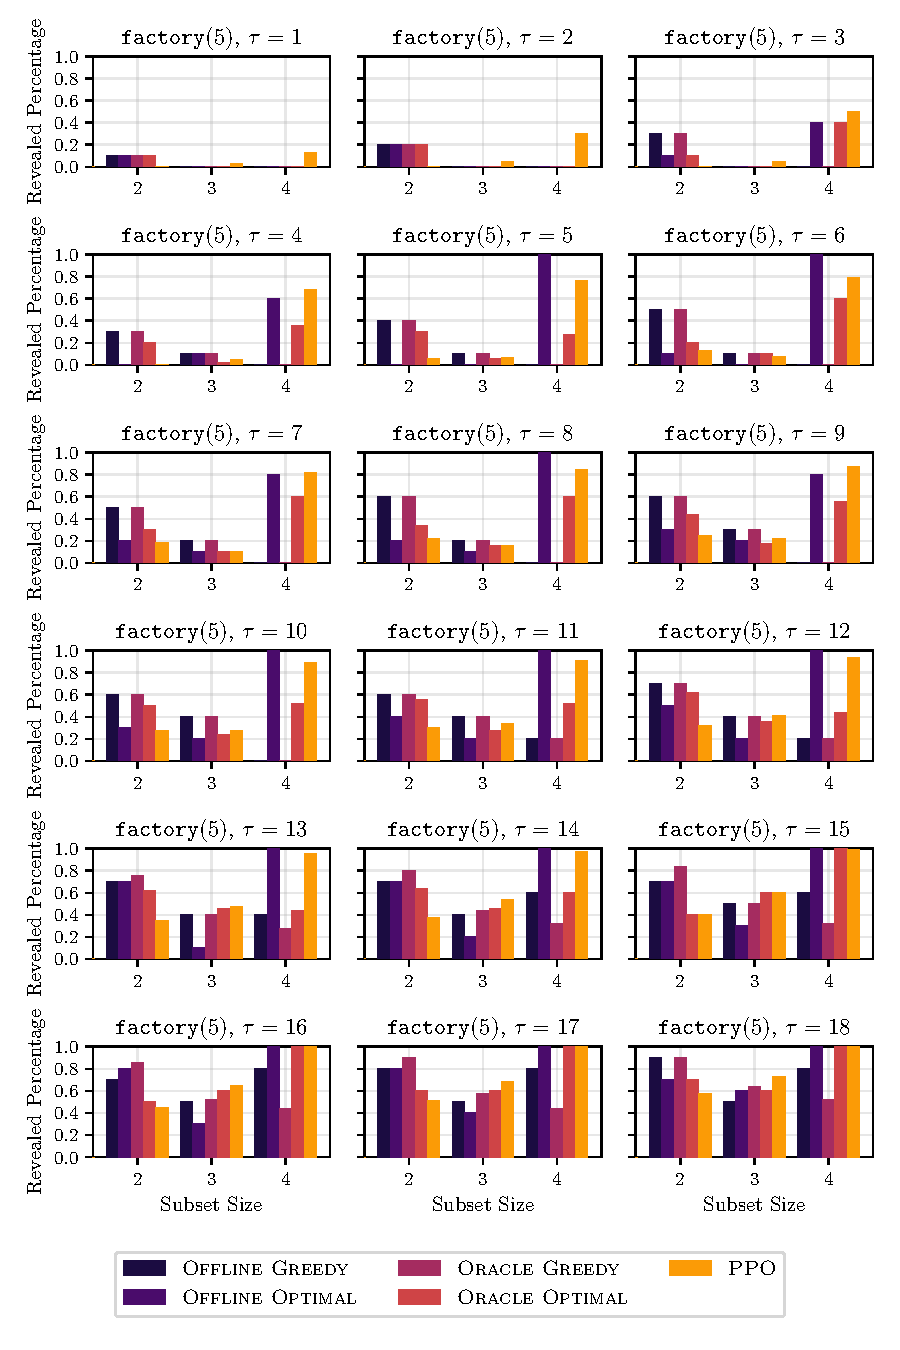
\includegraphics[width=\textwidth]{figures/linf_norm_predictible_factory5_coalition_bar_sizes.pdf}
	\caption{ The percentage of subsets of a given size revealed in steps $1 $ to $ 25 $ for the different approaches, when ran on the $\factory[5]$ distribution with $L_\infty$-divergence.}
	\label{fig:factory_linf_coals}
\end{figure*}


% re-introduce what it's about
In \Cref{chap:pp}, we have proven various statements about the relationship between the solutions of the \algFO{} and \algRO{} algorithms, along with the relationships of the optimal algorithms and their greedy counterparts.
The last relationship we have not mentioned yet is that of \algFG{} and \algRG{}.
One might expect that the resulting valuation of \algFG{} would be an upper bound on \algRG{}, as was the case with their optimal variants.
The results we have presented thus far would seem to support this conclusion.
However, as we show in \Cref{fig:offlinebeatsoracle}, it is \emph{not} true in general.

% explain l-inf
Our counter-example uses the $ L_\infty $-divergence, working with the $ \factory $ distribution of functions, which is defined as \[
  \fce {L_\infty} x \deq \max_i \absolute{x_i}.
\]
The $ L_\infty $ norm is what the $ L_k $ norms converge to as $ k $ becomes large.
The performance of all our approaches on the $L_\infty$ norm is very different to what we saw in \Cref{fig:factory}.
Most notably, the performance of both the greedy algorithms is significantly worse than all the other approaches.
Around $ \tau = 10 $, they are both outperformed by even the \algRand{} benchmark.
Furthermore, the offline variant outperforms the oracle variant for some choices of $ \tau $.

% explain why
This is a direct consequence of our specific implementation, in particular, the tie breaking of our $ \argmin $ function.
Importantly, revealing any value at the start does not affect the value of the divergence.
In this case, our implementation of $ \argmin $ simply chooses the \textquote{first} action (in some internal ordering of actions it has, see \Cref{app:code} for further details).
Consequently, the greedy algorithms choose their first actions completely blindly.
Then, at $ \tau=15 $, the fact that \algFG{} sees an \emph{average} divergence of its actions in fact helps it make a better decision than \algRG{}, which just sees the effect of the action on the specific instance.

% btw ppo
Notice also that in this example, the PPO algorithm does not suffer from the same problem as the greedy approaches. 
In fact the PPO reaches performance comparable to the \algRO{} approach.

\section{Largest Coalition Heuristic}
\label{ssec:largest}

\begin{figure*}[t!]
  \centering
	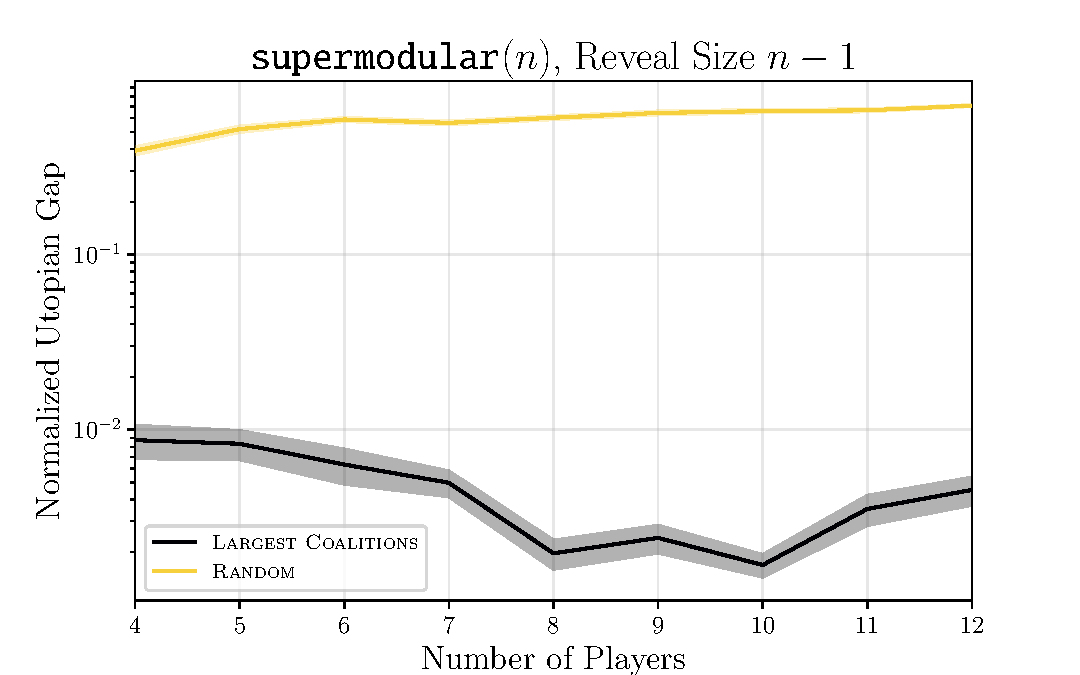
\includegraphics[width=\stdfigwidth]{figures/exploitability_convex_linear.pdf}
	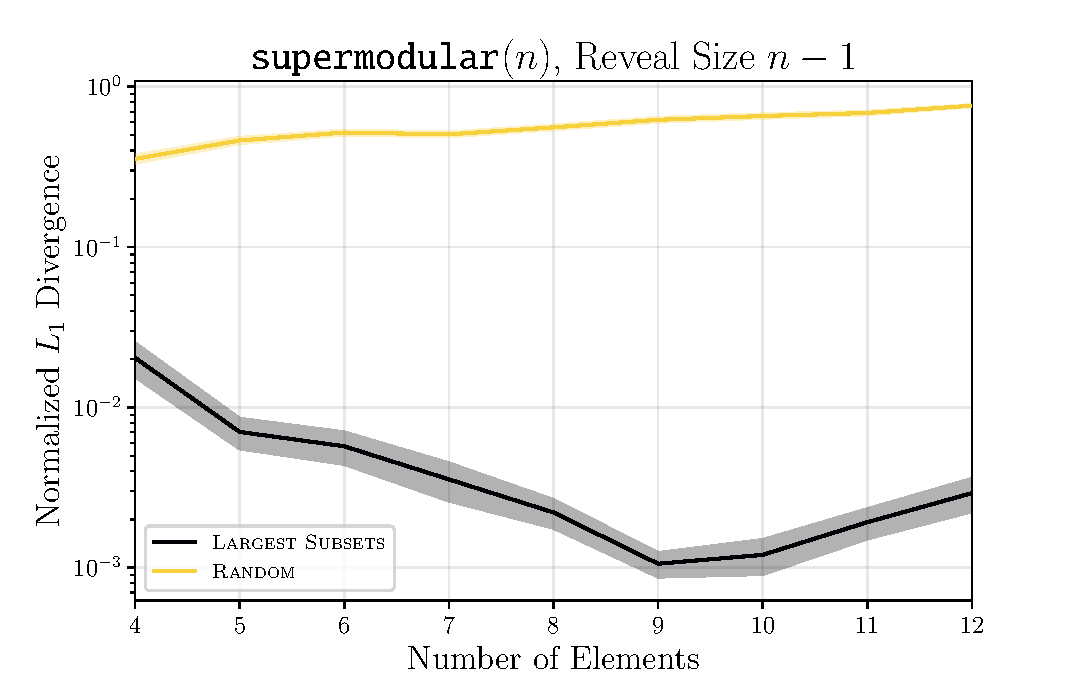
\includegraphics[width=\stdfigwidth]{figures/l1_norm_convex_linear.pdf}
	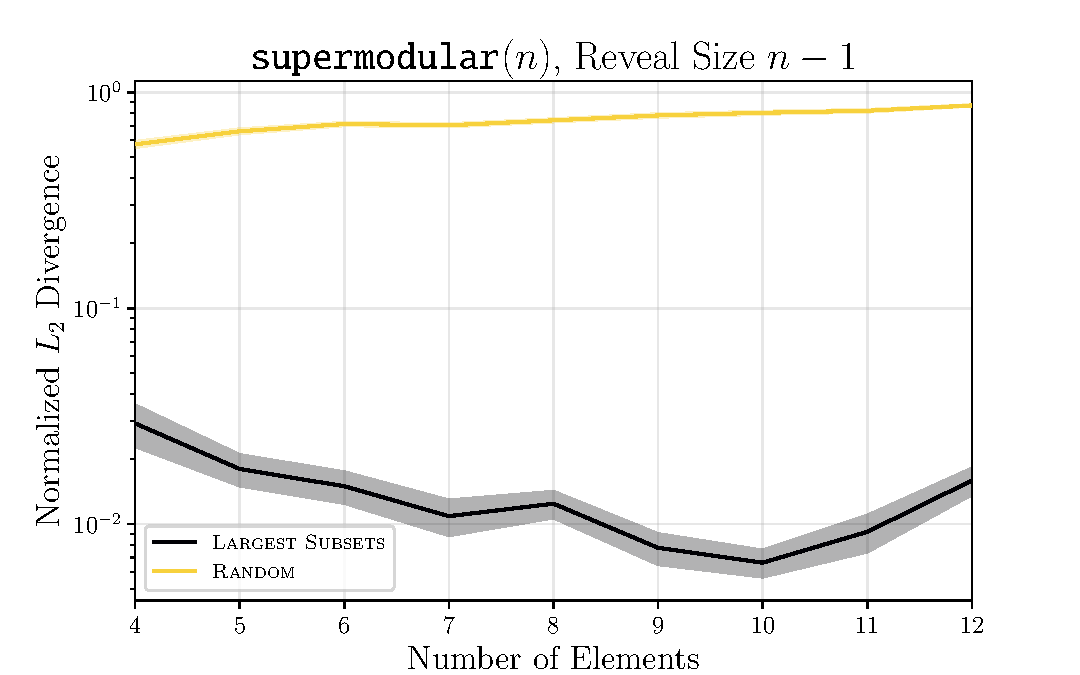
\includegraphics[width=\stdfigwidth]{figures/l2_norm_convex_linear.pdf}
	\caption{ The divergence as a function of budget $ \tau $ on the $ \supermodular $ distribution for the normalized utopian gap \citep[][Figure 3]{uradnik2024reducing} and the normalized $ L_1 $-divergence.}
	\label{fig:largest}
\end{figure*}

% explain motivation
The main motivation of this thesis is to find out which subsets/coalitions are in some sense the most important for a given distribution of set functions/cooperative games.
To do this for any given distribution of superadditive set functions, we have devised the algorithms described in \Cref{chap:pp}.
For some distributions, these algorithms are more effective at extracting the important subsets, while for others they are nearly comparable to revealing the subsets at random. % TODO: cycle dist? nebo tohle smazat?

In this section, we further investigate the $ \supermodular $ distribution, and we hypothesize about the generalization of what we have seen in our experiments for larger $ n $.
As we have seen in \Cref{fig:supermodular,fig:supermod_coals}, for $ n=5 $, all algorithms perform well while behaving all in a very similar way.
They all first choose the $ n $ largest subsets, after which the divergence decreases by about 99\% (depending on the choice of $ \ell $).

% comment on performance
This suggests that the \textquote{most important subsets} for the supermodular functions, at least in terms of the divergence, are in fact the largest subsets, in addition to the minimal information $ \k_0 $.
We thus propose the heuristic we call the \algLC{}, which, for a budget of $ \tau = n $, reveals the subsets $ \k = \k_0 \cup \left\{ N \setminus \left\{ i \right\} \suchthat i \in N \right\} $.
Unfortunately, we cannot compare this heuristic to the optimal algorithms for $ n > 5 $,  due to their time complexity (\Cref{thm:algfo-time-complexity-poly-tau}).
We hence compare it only with the \algRand{} strategy.
\Cref{fig:largest} shows the performance of this heuristic as a function of $ n $, with the utopian gap and the $ L_1 $-divergence.
In order to make the results comparable, we normalize the results by the initial divergence (utopian gap), i.e., $ \k = \k_0 $ for each $n$.

% explain why
Surprisingly, while the normalized divergence increases for the \algRand{} strategy as $ n $ grows, for our \algLC{} heuristic it stays the same, or even decreases.
In other words, while a random subset structure of size $ n $ carries \textquote{less information} as $n$ grows, the largest subsets get \textquote{more important} (again, in terms of the divergence).
We can thus reduce the gap to near-zero, while keeping the number of revealed subsets \emph{linear} in $ n $, instead of the exponentially many of them we would require to know the entire function.

To better understand why that is the case, we have analyzed the average values of subsets in the $ \supermodular $ distribution for the values of $ n \leq 12 $ presented in \Cref{fig:largest}.
We have found that, for any fixed $ n $, the average value of its subset decreases by several orders of magnitude as the size of the subset decreases.
This explains the good performance of our heuristic, as choosing large subsets limits the upper superadditive bounds of the smaller subsets the most.
